\documentclass[../main]{subfiles}
\begin{document}

\chapter{Private key authentication schemes}

\section{Difference between secrecy and authentication}

\begin{figure}[h]
    \centering
    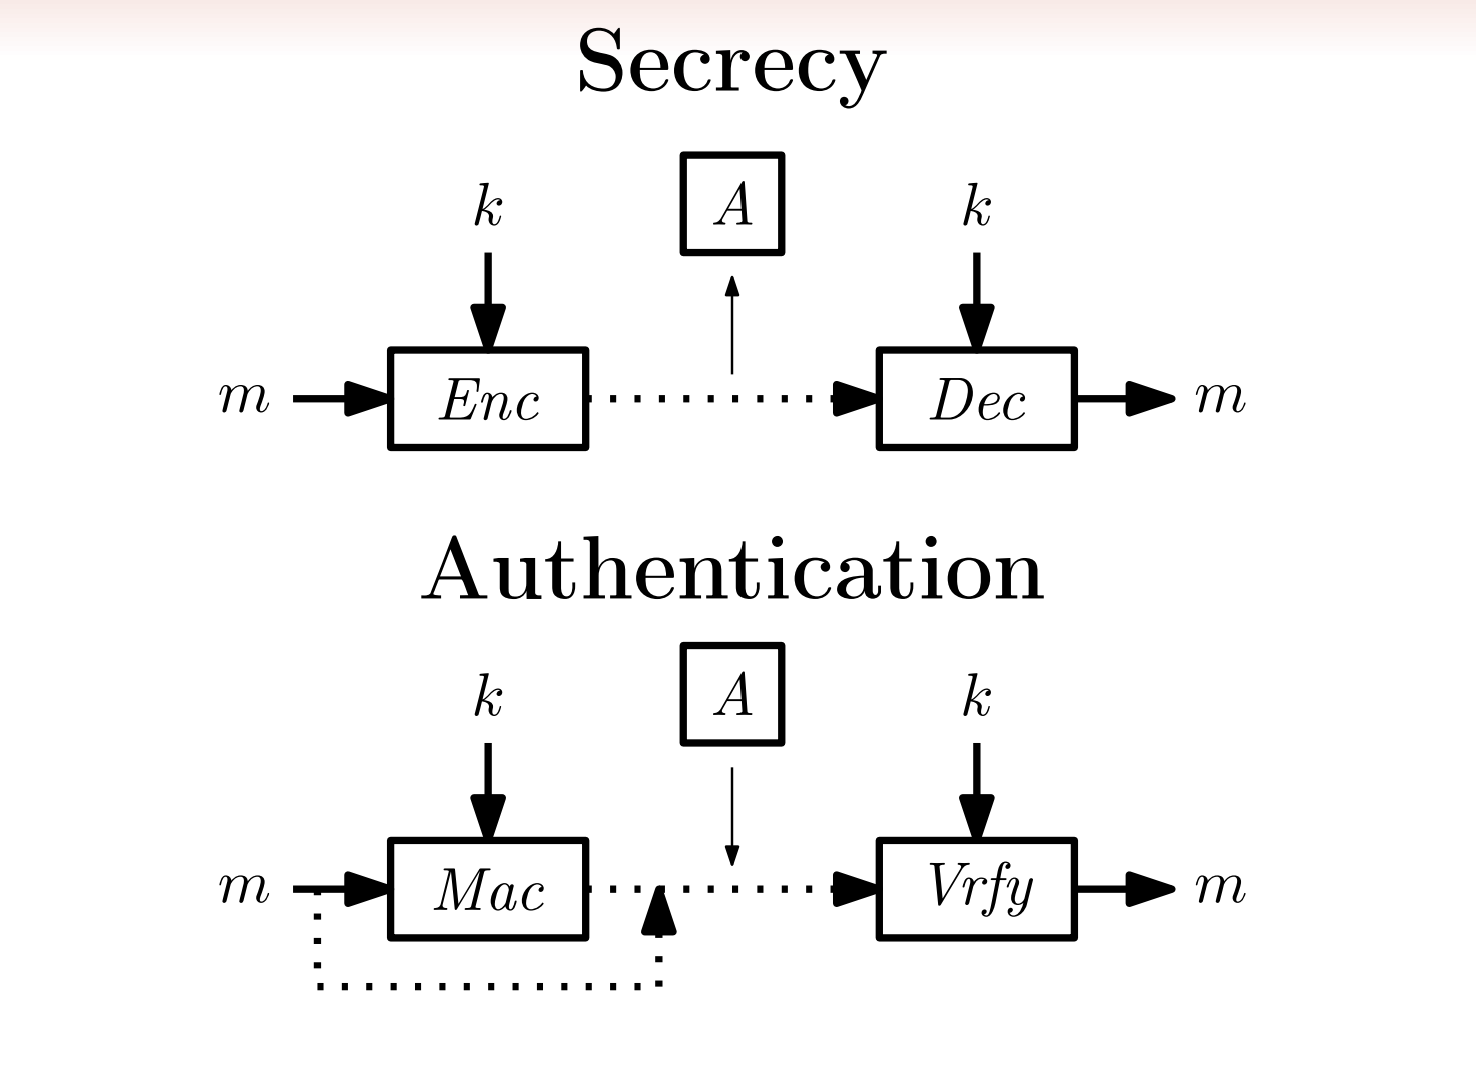
\includegraphics[width=0.5\textwidth]{images/difference_secrecy_authentication}
    \caption{Difference between secrecy and authentication.}
\end{figure}
\noindent
In \textbf{secrecy schemes}, the channel is secure and the focus of the adversary is reading what goes through the channel. 
In \textbf{authentication schemes}, the channel is not secure and the focus of the adversary is not to read the content of the channel, but to write on it.
That is why the receiver wants to be sure that the message sent along the channel is actually coming from the expected sender.
For that we need a \textbf{Message Authentication Code (MAC)}.\\
\noindent
Authentication and secrecy are different: solving the problem of secrecy does not solve the problem of authentication.
We do not want adversaries to be able to \textit{forge} messages of their choice $m$ without knowing a key $k$.

\section{Message Authentication Codes}
The same way ciphers guarantee secrecy, \textbf{Message Authentication Codes (MACs)} guarantee authentication.
\begin{definition}
    A MAC is a triple $\Pi = (Gen, Mac, Vrfy)$ of PPT algorithms such that:
    \begin{itemize}
        \item $Gen$ takes as input a string in the form $1^n$ (the security parameter) and outputs a key $k$ which can be such that $|k|\ge n$.
        \item $Mac$ takes as input a key $k$ and a message $m$ and outputs a \textbf{tag} $t$.
        \item $Vrfy$ takes as input a key $k$, a message $m$ and a tag $t$, and outputs a boolean $b$ (i.e., $b \in{} \{0,1\}$).
    \end{itemize}
    A MAC $\Pi = (Gen, Mac, Vrfy)$ is \textit{correct} when $Vrfy(k, m, Mac(k, m)) = 1$.
\end{definition}

\noindent
In order to be safe and sound, the assumptions are very pessimistic:
\begin{itemize}
    \item the adversary $A$ has access to an oracle $Mac_k(\cdot)$ which can be used to generate all possible tags;
    \item having access to a previously generated pair ($m$,$t$) is not interesting;
    \item $A$ has to be PPT;
    \item the new experiment is called $MacForge_{A,\Pi}(n)$.
\end{itemize}

\noindent
Let us present the new experiment:\\
$MacForge_{A,\Pi}(n):$\\
$k \leftarrow{} Gen(1^n)$\\
$(m,t) \leftarrow{} A(1^n,Mac_k(\cdot)) \;\;\;\;\;\;\;\;\;\;\;\;\;\;\;\;\;\;\;\;\;\; \text{// Invoked once.}$\\
$\mathbb{Q} \leftarrow \{m \; | \; A \text{ queries } Mac_k(\cdot) \text{ on } m\} \;\;\; \text{// Set of queries already performed by MacForge.}$\\
$\textbf{Result:} (m \notin{\mathbb{Q}} \wedge{} Vrfy(k,m,t) = 1) \;\; \text{// $m$ must be new and $Vrfy$ must succeed.}$

\begin{definition}
    A MAC $\Pi$ is secure if and only if for every PPT adversary $A$ there exists a function $\varepsilon{} \in{} \mathcal{NGL}$ such that:
    $$Pr(MacForge_{\Pi,A}(n) = 1) = \varepsilon(n)$$
\end{definition}
%----------------------------------------------------------------------------------
\subsection{Constructing a secure MAC}
\begin{definition}[FP induced MAC]
    Given an FP $F$, the MAC $\Pi{}^F = (Gen, Mac, Vrfy)$ is defined as follows:
    \begin{itemize}
        \item The algorithm $Gen$ for input $1^n$ outputs every string long $n$ with same probability, i.e. $\frac{1}{2^n}$.
        \item $Mac(k,m) = F_k(m)$.
        \item $Vrfy(k,m,t) = (F_k(m)\stackrel{?}{=}t)$ (it is $1$ (true) if and only if $F_k(m)$ equals $t$).
    \end{itemize}
\end{definition}

\begin{theorem}
    If $F$ is pseudorandom, then the MAC $\Pi{}^F$ is secure.
\end{theorem}

\paragraph{Proof}
Let's start by introducing an auxiliary MAC $\Tilde{\Pi}$ as follows:
\begin{itemize}
    \item $\Tilde{Gen}$ on input $1^n$ does not generate a key but a random function $f: \{0,1\}^n \rightarrow{} \{0,1\}^n$;
    \item $\Tilde{Mac}$ and $\Tilde{Vrfy}$ works pretty much like the corresponding algorithms in $\Pi{}^F$
\end{itemize}
First of all, observe that $\Tilde{\Pi}$ is secure: since $f$ is a function and the adversary is required to output a valid pair $(m,t)$ ($m \notin{} \mathbb{Q}$),
we are basically asking the adversary to guess a random string, namely $f(m)$. This probability is $\frac{1}{2^n}$.
As a consequence:
$$Pr(MacForge_{\Tilde{\Pi},A}(n) = 1) = \frac{1}{2^n}$$
Now, let's prove that the behaviour of any adversary $A$ against $\Tilde{\Pi}$ and $\Pi^F$ cannot be too different, i.e.,
$$|Pr(MacForge_{\Tilde{\Pi},A}(n) = 1) - Pr(MacForge_{\Pi^F,A}(n) = 1)| \le{} \varepsilon(n)$$
with $\varepsilon \in{} \mathcal{NGL}$.\\
We can construct a distinguisher $D_A$ by exploiting the adversary $A$ as follows:
\begin{figure}[H]
    \centering
    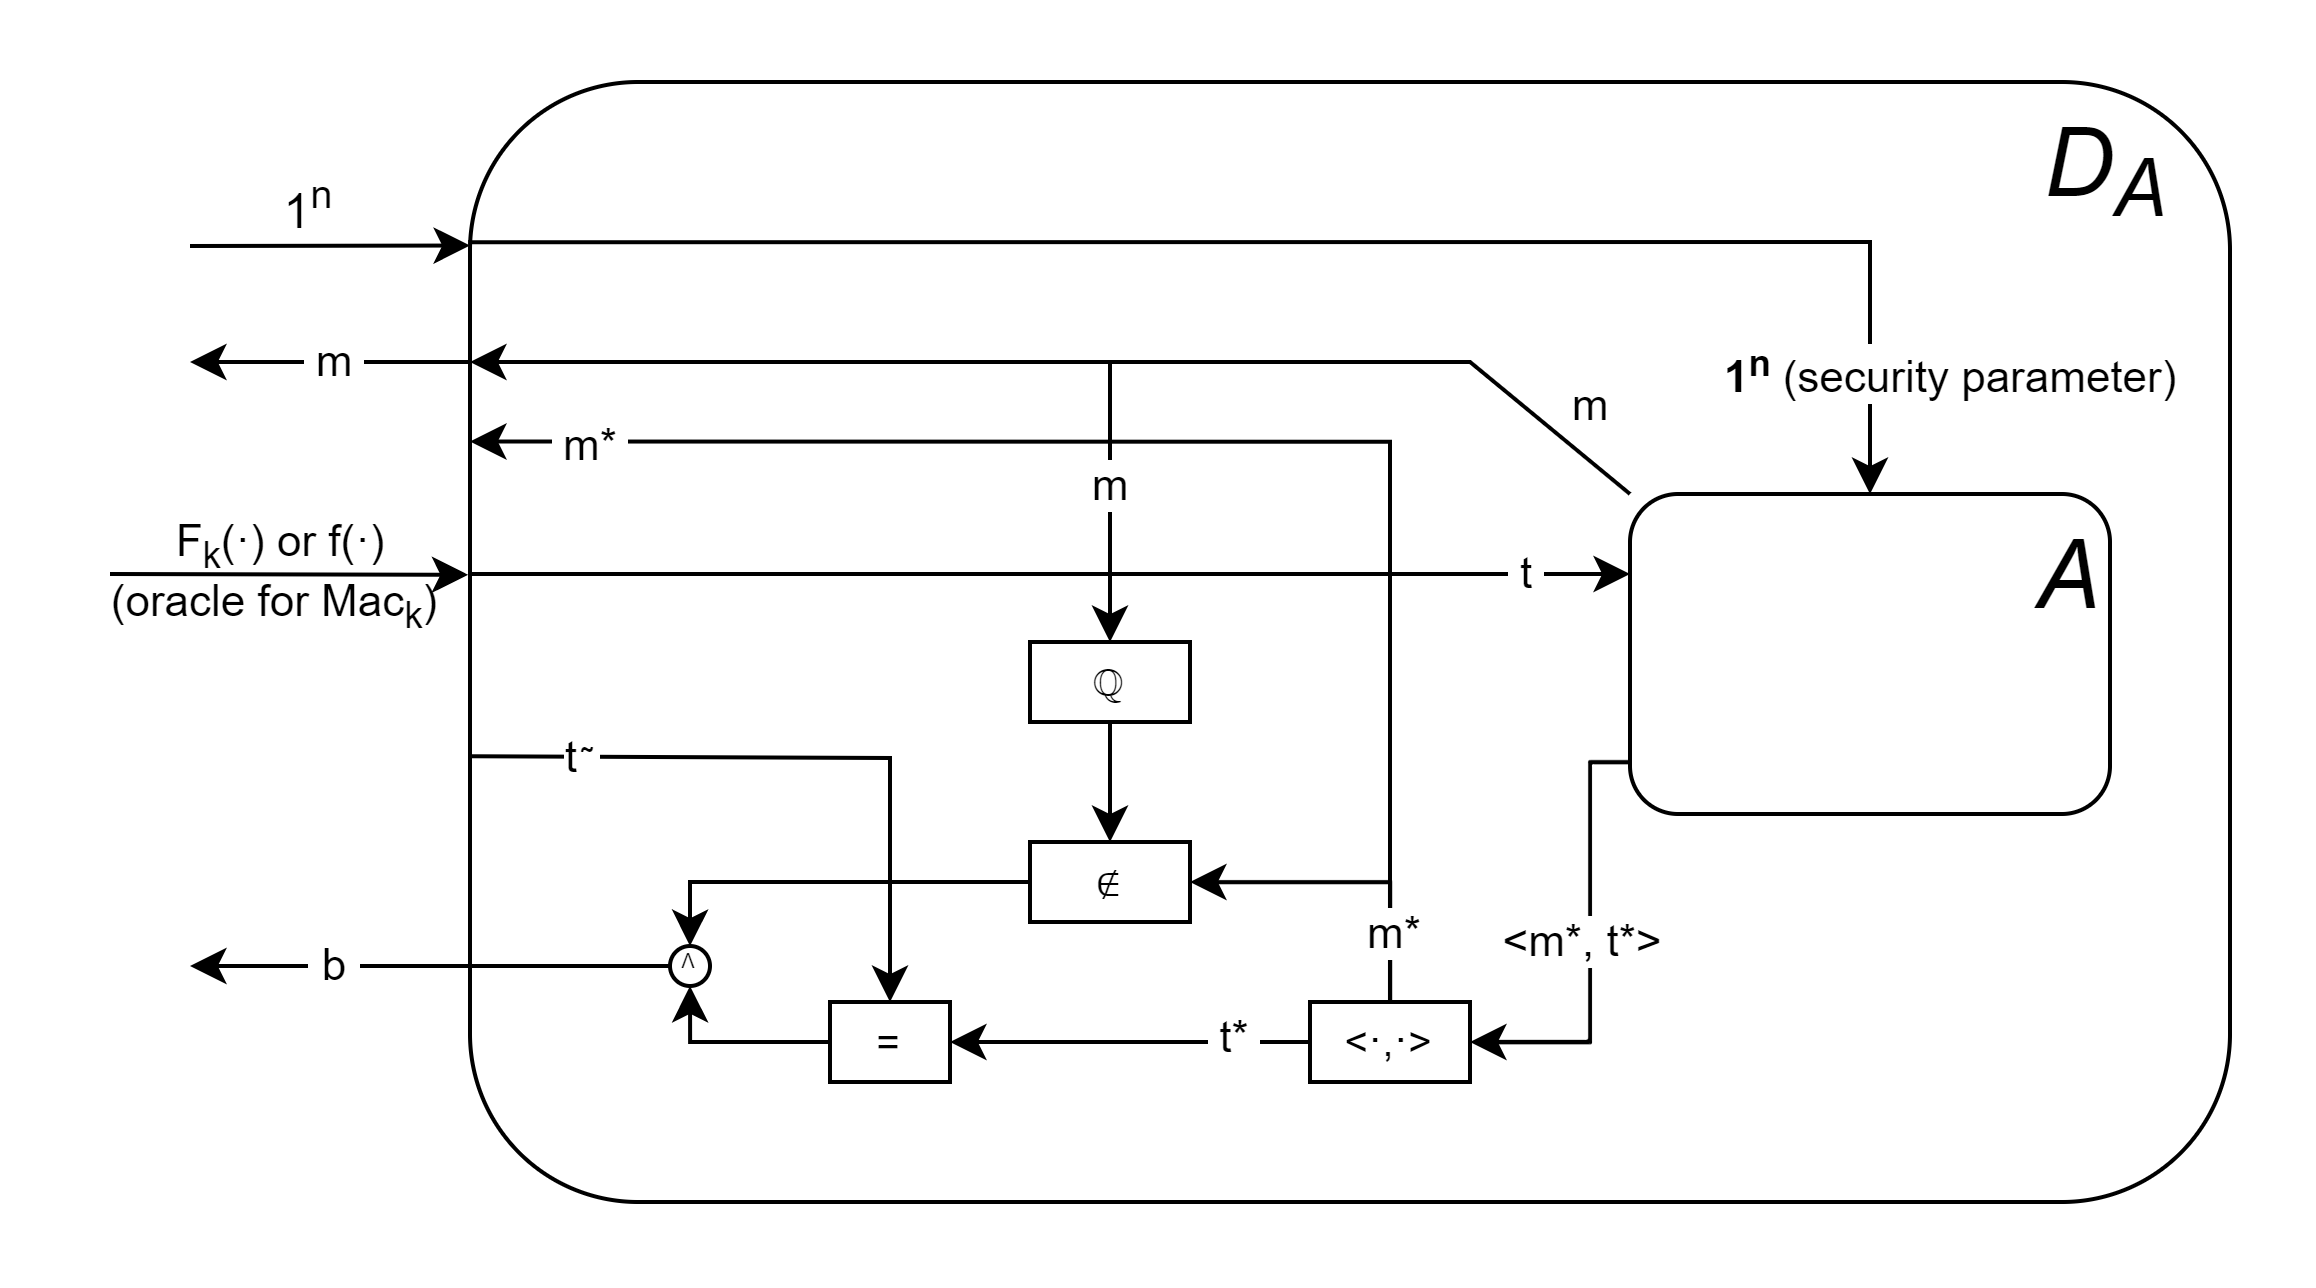
\includegraphics[width=0.8\textwidth]{images/security_of_mac_given_pseudorandom_F}
    \caption{How a distinguisher $D_A$ can be generated out of an attacker $A$.}
\end{figure}

\noindent
By this construction of $D_A$ we notice the following:
$$Pr(MacForge_{\Tilde{\Pi},A}(n) = 1) = Pr(D_A^{f(\cdot)}(1^n) = 1)$$
$$Pr(MacForge_{\Pi^F,A}(n) = 1) = Pr(D_A^{F_k(\cdot)}(1^n) = 1)$$
Since $F$ is pseudorandom, then we can prove what we wanted, that is:
$$|Pr(D_A^{f(\cdot)}(1^n) = 1) - Pr(D_A^{F_k(\cdot)}(1^n) = 1)| \le{} \varepsilon(n)$$
$$\Updownarrow$$
$$|Pr(MacForge_{\Tilde{\Pi},A}(n) = 1) - Pr(MacForge_{\Pi^F,A}(n) = 1)| \le{} \varepsilon(n)$$
%----------------------------------------------------------------------------------
\subsubsection{Handling Variable-Length messages}
$Mac^{*}(k, m)$:\\
$m_1 \mid\mid{} \ldots{} \mid\mid{} m_d \; \leftarrow{} \; m$\\
$\ell{} \; \leftarrow{} \; \mid{} m \mid{}$\\
\textbf{//such that $\mid{} m_i \mid{} = \frac{\ell{}}{4}$}\\
$r \; \leftarrow{} \; \{0, 1\}^{\frac{n}{4}}$\\
$\textbf{for} \; i \; \leftarrow{} \; 1 \; \textbf{to} \; d \; \textbf{do}$\\
$\quad{}\quad{} t_i \; \leftarrow{} \;$\\
$\quad{}\quad{}\quad{} Mac(k, r\mid\mid{}\ell\mid\mid{}i\mid\mid{}m_1)$\\
\textbf{Result}: $(r, t_1, \ldots{},t_d)$
\newline
\newline
$Vrfy^{*}(k, m, (r, t_1, \ldots{}, t_d))$:\\
$m_1 \mid\mid{} \ldots{} \mid\mid{} m_d \; \leftarrow{} \; m$\\
$\ell{} \; \leftarrow{} \; \mid{} m \mid{}$\\
\textbf{//such that $\mid{} m_i \mid{} = \frac{\ell{}}{4}$}\\
$\textbf{for} \; i \; \leftarrow{} \; 1 \; \textbf{to} \; d \; \textbf{do}$\\
$\quad{}\quad{} \textbf{if}$\\
$\quad{}\quad{}\quad{} Vrfy(k, r\mid\mid{}\ell\mid\mid{}i\mid\mid{}m_1) = $\\
$\quad{}\quad{}\quad{} 0 \; \textbf{then}$\\
$\quad{}\quad{}\quad{}\quad{}$ \textbf{Result}: 0\\
\textbf{Result}: 1

\begin{theorem}
    If $\Pi{}$ is secure, then $\Pi{}^*$ is also secure.
\end{theorem}
%----------------------------------------------------------------------------------
\subsubsection{CBC-MAC construction}
$Mac^{CBC}(k, m)$:\\
$\ell{} \; \leftarrow{} \; \ell{}(\mid{} k \mid)$\\
$m_1 \mid\mid{} \ldots{} \mid\mid{} m_{\ell} \; \leftarrow{} \; m$\\
\textbf{//such that $\mid{} m_i \mid{} = \; \mid{}k\mid{}$}\\
$t_0 \; \leftarrow{} \; 0^n$
$\ell{} \; \leftarrow{} \; \mid{} m \mid{}$\\
$\textbf{for} \; i \; \leftarrow{} \; 1 \; \textbf{to} \; \ell{} \; \textbf{do}$\\
$\quad{}\quad{} t_i \; \leftarrow{} \; F_k(t_{i-1} \oplus{} m_i)$\\
\textbf{Result}: $t_{\ell}$
\newline
\newline
$Vrfy^{*}(k, m, t)$:\\
\textbf{if} $\ell{}(\mid k \mid) \cdot{} \mid{} k \mid{} \neq{} \mid{} m \mid{}$ \textbf{then}\\
$\quad{}\quad{} \textbf{Result}: 0$\\
$\textbf{Result}: t \stackrel{?}{=} MAC^{CBC}(k, m)$\\

\begin{theorem}
    If $\ell{}$ is a polynomial and $F$ is $FP$, then $\Pi{}^{CBC}$ is a secure MAC.
\end{theorem}
%----------------------------------------------------------------------------------
\section{Hash functions}
\begin{definition}
    A hash function is a pair of PPT algorithms $(Gen, H)$ such that:
    \begin{itemize}
        \item Gen is an algorithm that takes as input a security parameter $1^n$ and return a key $s$ (from which $n$ can be efficiently calculated).
        \item There exists a polynomial $\ell{}$ such that $H(s, x)$ returns a string of length $\ell{}(n)$ (where $n$ is implicit parameter in $s$)
    \end{itemize}
\end{definition}
%----------------------------------------------------------------------------------
\subsection{Collision-Resistant hash functions}
$HashCol_{\mathcal{A}, \Pi{}}(n):$\\
$s \; \leftarrow{} \; Gen(1^n)$\\
$(x, y) \; \leftarrow{} \; A(s)$\\
\textbf{Result}: $(x \neq{} y) \wedge{} (H(x) = H(y))$

\begin{definition}
    A hash function $\Pi{} = (Gen, H)$ is collision-resistant if and only if for every adversary PPT $A$ there exists a negligible function $\varepsilon{}$ such that $$Pr(HashColl_{\mathcal{A}, \Pi{}}(n)=1) \leq{} \varepsilon{}(n)$$
\end{definition}
%----------------------------------------------------------------------------------
\subsubsection{Birthday attacks}
\begin{theorem}[Birthday theorem]
    Given $q$ uniformly chosen random values in a finite set of cardinality $N$, the probability that two of them are identical is $\frac{q^2}{N}$.
\end{theorem}
%----------------------------------------------------------------------------------
\subsubsection{The Merkle-Damgård transform}
$H^{MD}(s, x):$\\
$B \; \leftarrow{} \; \lceil{} \frac{\mid{}x\mid{}}{n} \rceil{}$\\
$x_1 \mid\mid{} x_B \; \leftarrow{} \; x$\\
\textbf{//such that $\mid{} x_i \mid{} = n$}\\
$x_{B+1} \; \leftarrow{} \; \mid{} x \mid{}$\\
$z_0 \; \leftarrow{} \; 0^n$\\
$\textbf{for} \; i \; \leftarrow{} \; 1 \; \textbf{to} \; B+1 \; \textbf{do}$\\
$\quad{}\quad{} z_i \; \leftarrow{} \; H(s, z_i - 1, \mid\mid{} x_i)$
\textbf{Result}: $z_{B+1}$

\begin{theorem}
    If $(Gen, H)$ is collision-resistant, then so is $(Gen, H^{MD})$.
\end{theorem}
%----------------------------------------------------------------------------------
\subsubsection{Hash-and-Mac}
\begin{theorem}
    If $\Pi{}$ is a secure MAC and $(Gen', H)$ is collision-resistant, then $\Pi{}^H$ is secure. 
\end{theorem}

% \paragraph{Proof}
\end{document}